\subsubsection{Total number of collisions}\label{subsubsec:rect2krcollisions}

For the total number of collisions we get a very low unexplained variation
(\(0.72\%\)). The broadcast radius accounts for the \(64.31\%\) of the variation
and it is the dominant factor, as in other scenarios. As in the low density
scenario and differently from the high density one, the second most important
factor was the maximum number of copies, which accounts for the \(16.47\%\) of
the variation while the maximum relay delay (third factor) accounts only for the
\(4.86\%\) of the variation. In this case, also the combination of the broadcast
radius and the maximum number of copies is relevant (\(9.59\%\)). This results
are not surprisingly because the density of the rectangular scenario is the same
as the low density one (which is a square).

As in the case of other configurations, we need to decrease the broadcast radius
to reduce the total number of collision, which is an obvious consideration, and
as shown in \figref{fig:rectperfcollisionsm} using lower values for the maximum
number of copies reduces the total number of collisions.

The fact that the broadcast radius is less important in this scenario compared
to the high density case, but more important with respect to the low density,
can be explained by the fact that the users are scattered in the floorplan, so
we need a huger increase of the broadcast radius to see an effect, but they are
not so well distributed because they are flattened in the rectangle.

\begin{figure}[htb]
	\centering
	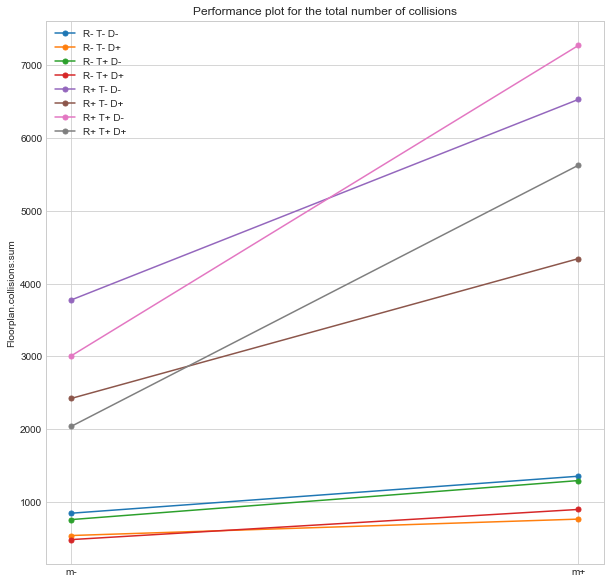
\includegraphics[width=\textwidth]{img/rect/collisions_m_perfplot.png}
	\caption{Decrease the maximum number of copies to decrease the total
	number of collisions}\label{fig:rectperfcollisionsm}
\end{figure}
